\documentclass[tikz,border=3mm]{standalone}
\usepackage{tikz}
\usetikzlibrary{positioning}

\begin{document}

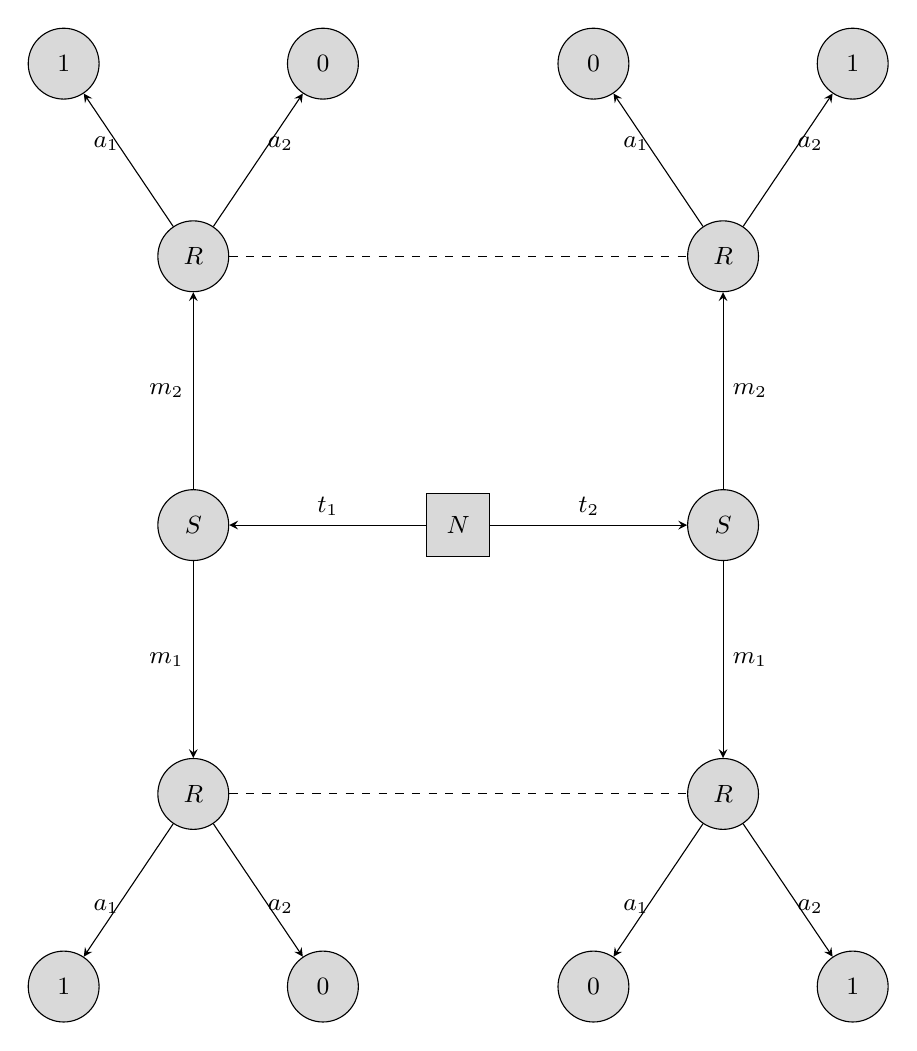
\begin{tikzpicture}[
  every node/.style={font=\small},
  state/.style={circle,draw,fill=gray!30,minimum size=9mm,inner sep=0pt},
  nature/.style={rectangle,draw,fill=gray!30,minimum size=8mm,inner sep=0pt},
  >=stealth
]

% NATURE
\node[nature] (N) at (0,0) {$N$};

% SENDERS
\node[state] (S1) [left=25mm of N] {$S$};
\node[state] (S2) [right=25mm of N] {$S$};

\draw[->] (N) -- node[above] {$t_2$} (S2);
\draw[->] (N) -- node[above] {$t_1$} (S1);

% RECEIVERS (middle row)
\node[state] (R1mid) [below=25mm of S1] {$R$};
\node[state] (R2mid) [below=25mm of S2] {$R$};

\draw[->] (S1) -- node[left]  {$m_1$} (R1mid);
\draw[->] (S2) -- node[right] {$m_1$} (R2mid);

% RECEIVERS (top row)
\node[state] (R1top) [above=25mm of S1] {$R$};
\node[state] (R2top) [above=25mm of S2] {$R$};

\draw[->] (S1) -- node[left]  {$m_2$} (R1top);
\draw[->] (S2) -- node[right] {$m_2$} (R2top);

% INFORMATION SETS
\draw[dashed] (R1mid) -- (R2mid);
\draw[dashed] (R1top) -- (R2top);

% ACTION OUTCOMES: middle row
\node[state] (R1a1) [below left=18mm and 10mm of R1mid] {$1$};
\node[state] (R1a2) [below right=18mm and 10mm of R1mid] {$0$};

\node[state] (R2a1) [below left=18mm and 10mm of R2mid] {$0$};
\node[state] (R2a2) [below right=18mm and 10mm of R2mid] {$1$};

\draw[->] (R1mid) -- node[below left]  {$a_1$} (R1a1);
\draw[->] (R1mid) -- node[below right] {$a_2$} (R1a2);

\draw[->] (R2mid) -- node[below left]  {$a_1$} (R2a1);
\draw[->] (R2mid) -- node[below right] {$a_2$} (R2a2);

% ACTION OUTCOMES: top row
\node[state] (R1Ta1) [above left=18mm and 10mm of R1top] {$1$};
\node[state] (R1Ta2) [above right=18mm and 10mm of R1top] {$0$};

\node[state] (R2Ta1) [above left=18mm and 10mm of R2top] {$0$};
\node[state] (R2Ta2) [above right=18mm and 10mm of R2top] {$1$};

\draw[->] (R1top) -- node[above left]  {$a_1$} (R1Ta1);
\draw[->] (R1top) -- node[above right] {$a_2$} (R1Ta2);

\draw[->] (R2top) -- node[above left]  {$a_1$} (R2Ta1);
\draw[->] (R2top) -- node[above right] {$a_2$} (R2Ta2);

\end{tikzpicture}

\end{document}
